
\section{Co-design of estimation and control}
\label{sec:codesign}
In a traditional control system, such as the one shown in Fig.~\ref{fig:traditionalCE}, the controller is unaware of the implementation details of the estimation module and the estimation module is unaware of the requirements of the controller. 
For example, the design of the controller might not take into account the fact that obtaining a state estimate from a video feed will take a non-negligible amount of time, which we refer to as the estimation delay.
Conversely, the design of the estimator might not take into account the varying real-time constraints that the controlled system must satisfy, and instead always use a fixed amount of time to compute its estimates.
In order to improve performance of over-loaded closed loop systems, we propose the \emph{co-design} of estimation and control. 
The co-design involves using a \emph{contract-based framework} for both estimator and controller.
Namely, the controller requests the estimator to provide a state estimate within a certain deadline $\delta$ seconds and with a certain error bound $\epsilon$.
We refer to the tuple $(\delta,\epsilon)$ as the \emph{contract} between controller and estimator.
The estimator then provides an estimate that respects the contract.
By requesting estimates with varying contracts during system operation, the controller is able to do real-time adaptation of the closed-loop system performance to the current condition of the physical system.
For example, it can detect when an estimate is needed fast (but usually with higher error), and when a more accurate estimate is needed (but with greater delay).
A high-level view of this setup is shown in Fig.~\ref{fig:codesignedCE}. 

To ensure that the estimator can respect the contract (alternatively, that the controller is only requesting contracts that can be fulfilled by the estimator), the estimator is profiled off-line.
Namely, the estimator's parameters are varied and for each setting of the parameters, it is run on a \emph{profiling data set}. 
This yields a set of $(\delta,\epsilon)$ values, each one corresponding to a setting of the parameters.
These values can be plotted on a curve, which we call the \emph{error-delay curve}, an example of which is shown in Fig.??.
The detailed procedure for obtaining such a curve for a wide range of visual state estimation algorithms is given in Section \ref{delayErrorCurve}.
%Section \ref{discussion} discusses the applicability of this contract-based approach to state estimation and further extensions.

Online, when the estimator receives a $\de$ contract request from the controller, it can adapt its execution paths to respect the contract, namely, to provide a state estimate within the requested error bound $\epsilon$, and within the requested deadline $\delta$.

In addition, the controller is designed with the knowledge of the error-delay curve of the estimation algorithm, and requests contracts from that curve.
Thus, the error-delay curve constitutes the interface between controller and estimator.
This gives the controller the ability to leverage the flexible nature of the estimation algorithm to maximize some performance measure while not being concerned about the internal workings of the estimator. 
This allows a co-design of control and estimation without violating the separability principle, which is key to the design of closed-loop control systems.

Fig.~\ref{fig:fullcodesignedCE} shows the closed loop architecture in a system with co-design of the perception and control algorithms. 
Unlike a closed loop system where the perception module is designed to operate at a fixed operating point, in the co-designed system, the controller can make the estimation algorithm switch to lower time/energy consuming modes based on the control objective at the current time step.
The main components of the co-design architecture are a contract time perception algorithm, a robust control algorithm that computes an input to be sent to the plant as well as the operating mode for the contract time perception algorithm, and the interface between them. More details on these components are in the following sections.

\begin{figure}[t]
	\centering
		\includegraphics[width=0.7\linewidth]{placeHolder}
		\label{fig:fullcodesignedCE}
		\caption{Co-design of contract-based controller and estimator.}			
\end{figure}

\subsection{contract based perception algorithms}

In order to maximize the efficiency of the computation and control system, a contract based perception algorithm can operate at different deadlines and provide a usable solution for the control algorithm to operate on. This flexible operation of the generally run-to-completion algorithms is achieved by composing the algorithm of functional blocks that have different computation times and result in different qualities of outputs. Note that this problem is different from that of composing anytime algorithms together. Anytime algorithms have a well defined computation time versus quality tradeoff, but in our case we are composing together blocks that are individually run-to-completion and in most cases do not have a well defined intermediate measurable quality.

Figure \ref{} shows an example where an object recognition algorithm is composed of different functional blocks of varying computation time and result in a different accuracy when linked provide the functionality of an object recognition algorithm, e.g. the pixel classifier could be a Gaussian Mixture Model with 3, 5, or 7 components, with more components providing better classification performance at the cost of more computation time. The output of the .... \textbf{<more details here>}. 

%This composition of individual components can be represented as a decision tree where edges are blocks of code and nodes are their intermediate outputs/input to the next stage. An extensive profiling stage at design time helps assign distributions for execution times to the edges and distributions for output quality to paths along the tree. At run-time, this knowledge of execution times and output quality distributions can be used to generate a composition to realize a given criteria. An example of a criteria is to maximise the expected quality while meeting the given deadline with a high probability $\eta$.  



%Given a decision tree with pre-profiled information about execution time distributions for edges and quality for paths, this optimization can be mapped to an integer programming problem for edge selection in the tree. This problem can be solved in a 

%\textbf{<more details on the optimization here>}

\subsection{Interface between contract based perception and robust control}

For the control algorithm to be able to leverage the flexible nature of the contract based perception algorithm, it must have information about the computation time versus output quality trade-off that the contract based perception algorithm offers, but should not be exposed to or made dependent on to too much detail on how the trade-off is obtained. An interface that achieves this is to simply represent the profiled behaviour of the contract based algorithm to varying deadlines, as points on a perception quality versus deadline ($\delta, \epsilon$) curve, e.g. in figure \ref{fig:eps_delta_toy}. 
With this profiled curve available to the controller at runtime, the exchange of information between the contract based perception algorithm and the control algorithm consists of the controller assigning a deadline ($\delta$), or a contract to the perception algorithm with an expected bound on the quality ($\epsilon$) of its output. The perception algorithm then returns an output after internally deciding the composition to best meet the deadline and the expected quality requirement. While in many systems, assigning a contract for time and simultaneously expecting a minimum quality output may be an infeasible proposition, in this paper we only consider settings where neither the $\delta$ contract nor the $\epsilon$ bound are violated. This helps in formulating a control algorithm that provides mathematical guarantees on the feasibility of constraints for the safe operation of the closed loop dynamic system.

\begin{figure}[t]
	\centering
	\includegraphics[width=0.7\linewidth]{figures/placeHolder}
	\caption{Profiled perception versus computation time curve.}
	\label{fig:eps_delta_toy}
\end{figure}

\subsection{Robust Control with contract based perception algorithm}

\textbf{<Talk about control requirements, cost function, constraints, and mpc/rmpc here>}
The control algorithm designed to pick the best operating point based on the current state of the dynamic system to maximize a performance measure while being robust to the varying computation time, which shows up as a delay to the control algorithm, and the varying quality of output, which are varying estimation errors to the controller.






